%%%%%%%%%%%%%%%%%%%%%%%%
%
%   Thesis template by Youssif Al-Nashif
%
%   May 2020
%
%%%%%%%%%%%%%%%%%%%%%%%%




\section{NHTSA Special Crash Investigations}
 For the NHTSA's Special Crash Investigation dataset, a hierarchical clustering was performed on the resulting graph kernel computed from the skip-gram graphs. Since this dataset was pretty small at $N=48$, it served as a good subject to study the interactions between modifying the skip window width, kernel hyper parameters, and number of clusters. This study on these interactions informs decisions made on which hyper parameters to use in final analysis of the NHTSA data as well as the reddit thread data. \\
 
For the study on these interactions, hyper-parameters were varied and the value of cluster within sum of squares was tracked. Specifically, the values in Figure 4.1 were tested. \\
 

\begin{figure}
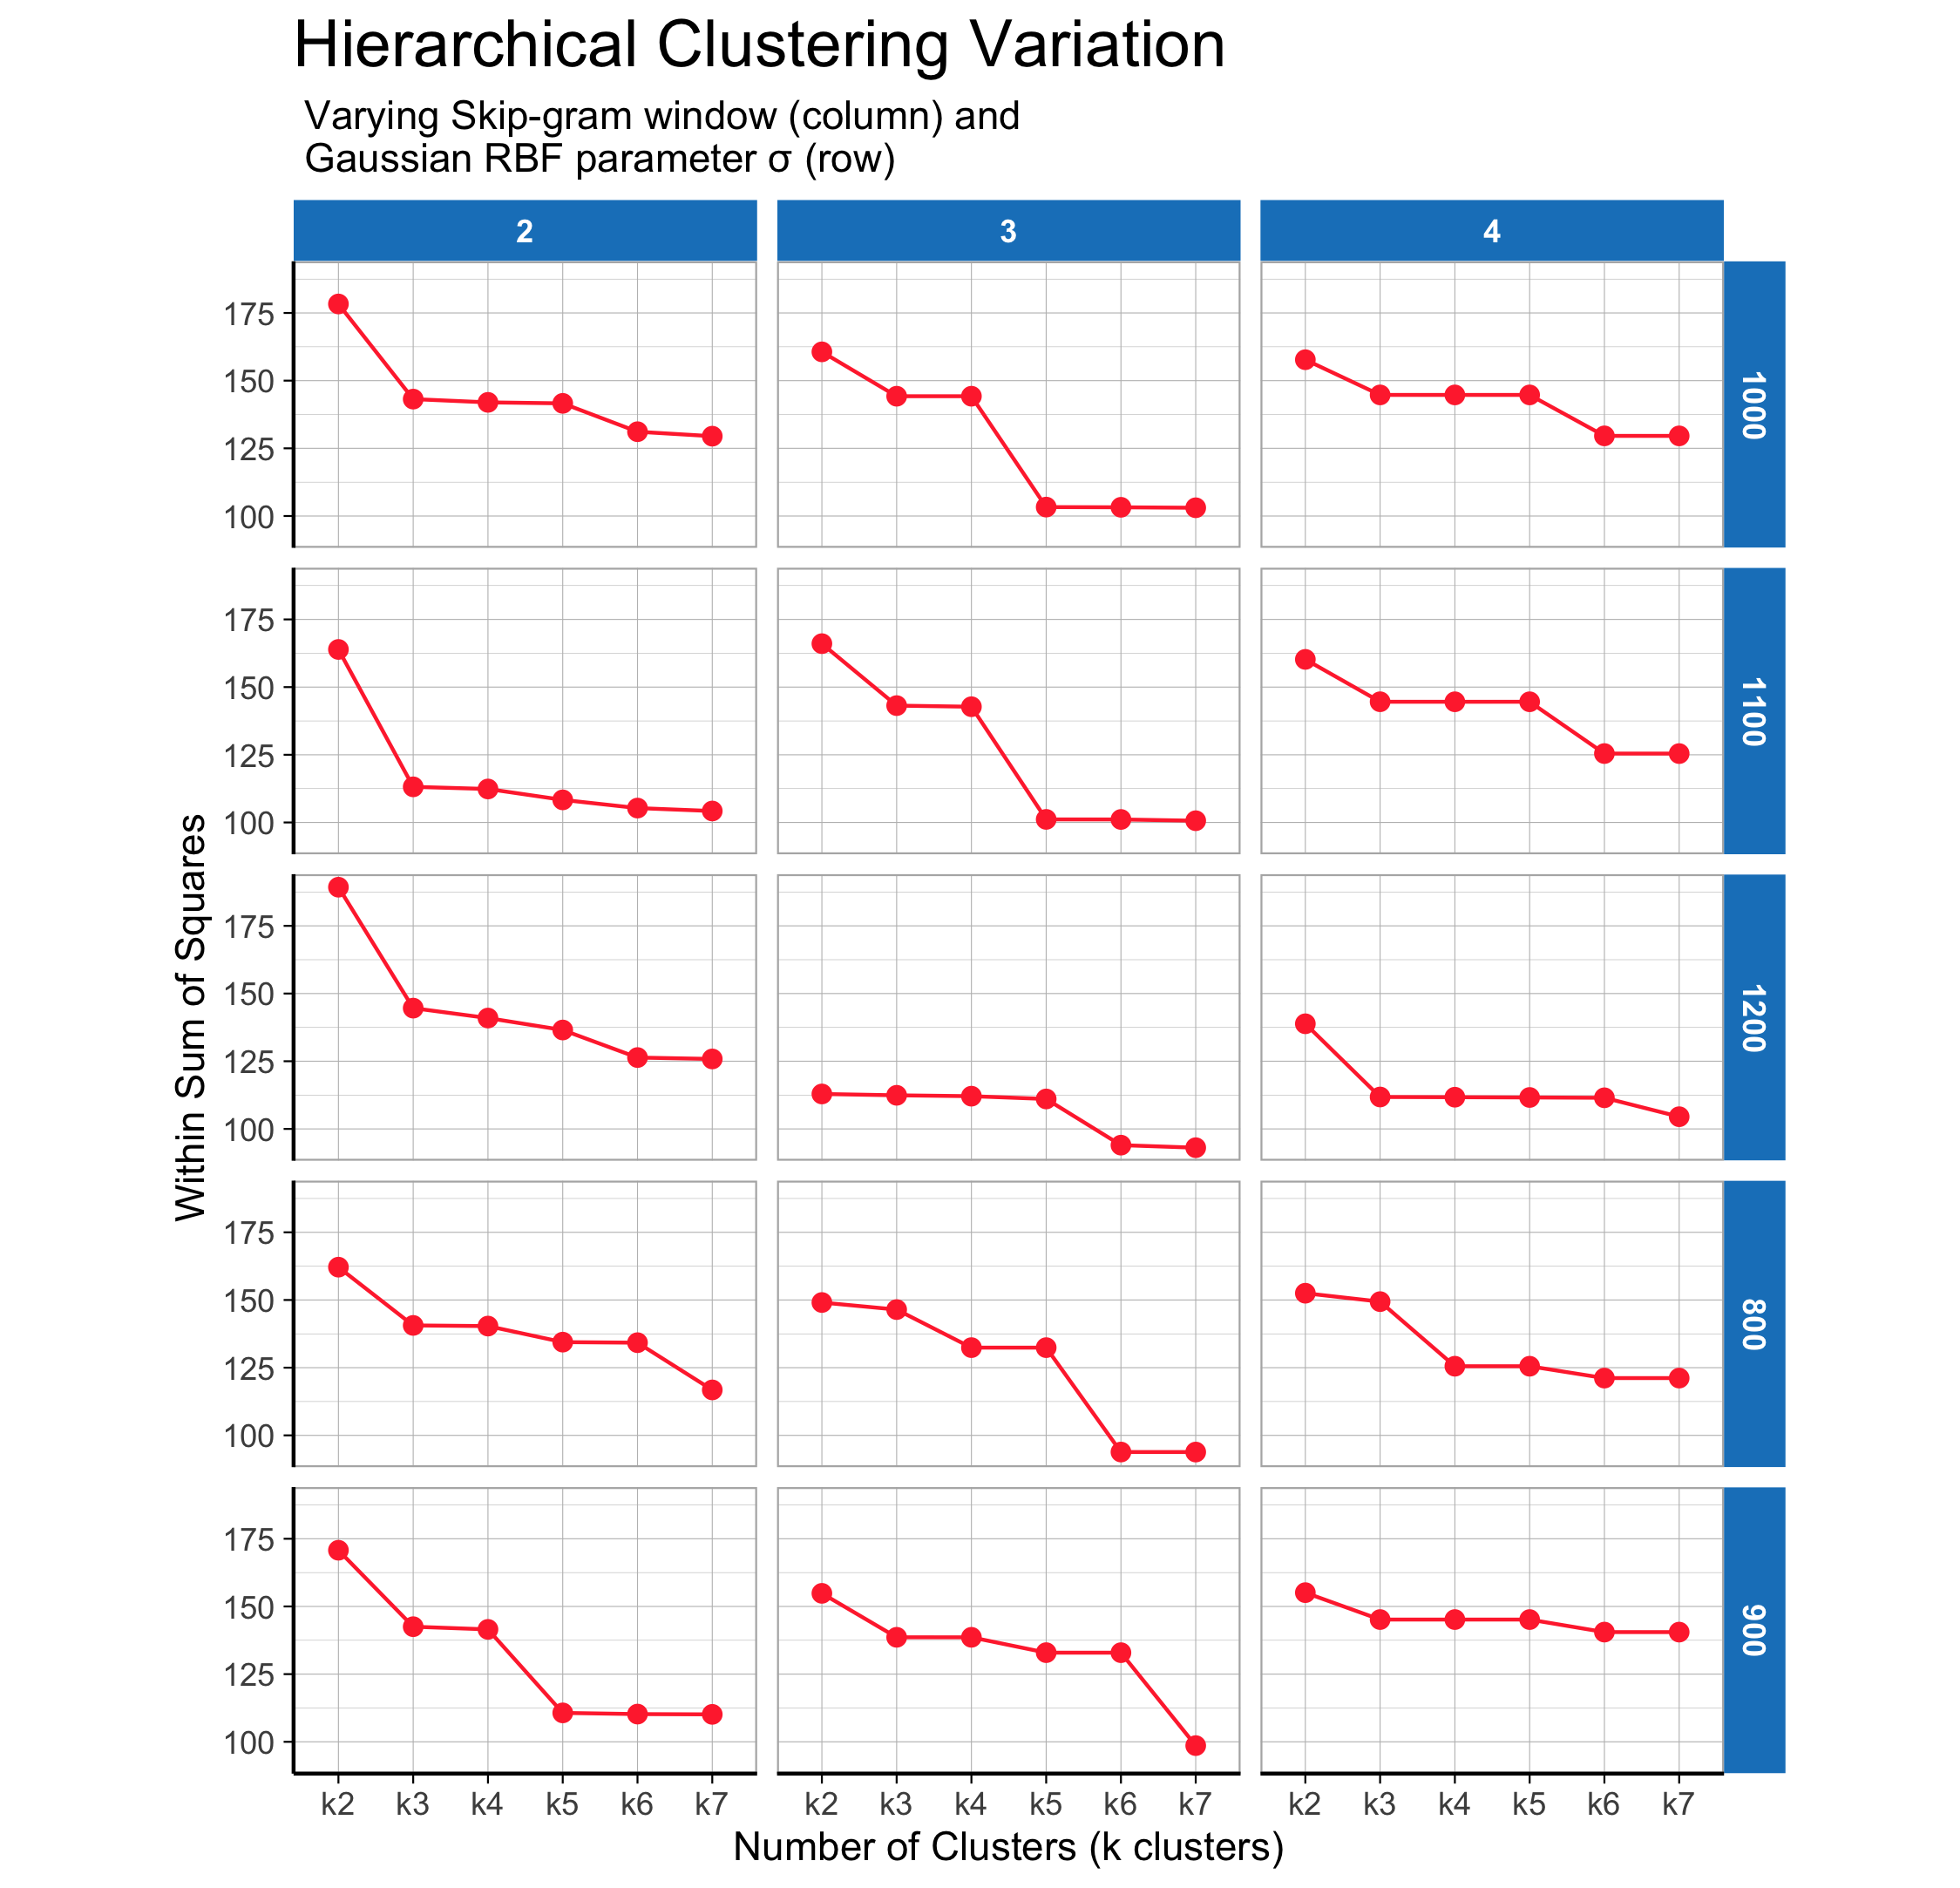
\includegraphics[width=6in]{Content/Images/hclust_variation.png}
\caption{Hierarchical Clustering Variation (NHTSA) for differing hyper-parameters.}
\end{figure}

In Figure 4.1, we see some promising values occurring at more prominent ``elbow" points in the plots. These points will be further analyzed and compared. The hyper parameters for these points are:\\

\begin{table}
\centering
\begin{tabular}{c|c|c|c}
Point&Skip-gram k& Graph Kernel sigma&No. of Clusters \\
\hline
A&3&1000&5\\
B&2&1100&3\\
C&3&1100&5\\
D&3&800&6\\
E&3&900&7
\end{tabular}
\caption{Hyper-parameter for Variation Study in Figure X}
\end{table}

These hyper-parameter sets, and their corresponding graph kernel matrix, are used in a hierarchical clustering analysis. The results from the analysis perform well, and display prominent clusters, often of comparable sizes.In Figure 4.2, we see the 5 dendrograms produced from hyper-parameter sets A,B,C,D, and E. Upon some examination, one will notice that documents often appear in the same clusters together, regardless of the hyper-parameter sets. This is most encouraging, as it indicates that these clusters are not a result of user-chosen parameters, but that the documents are indeed similar. \\

\begin{figure}
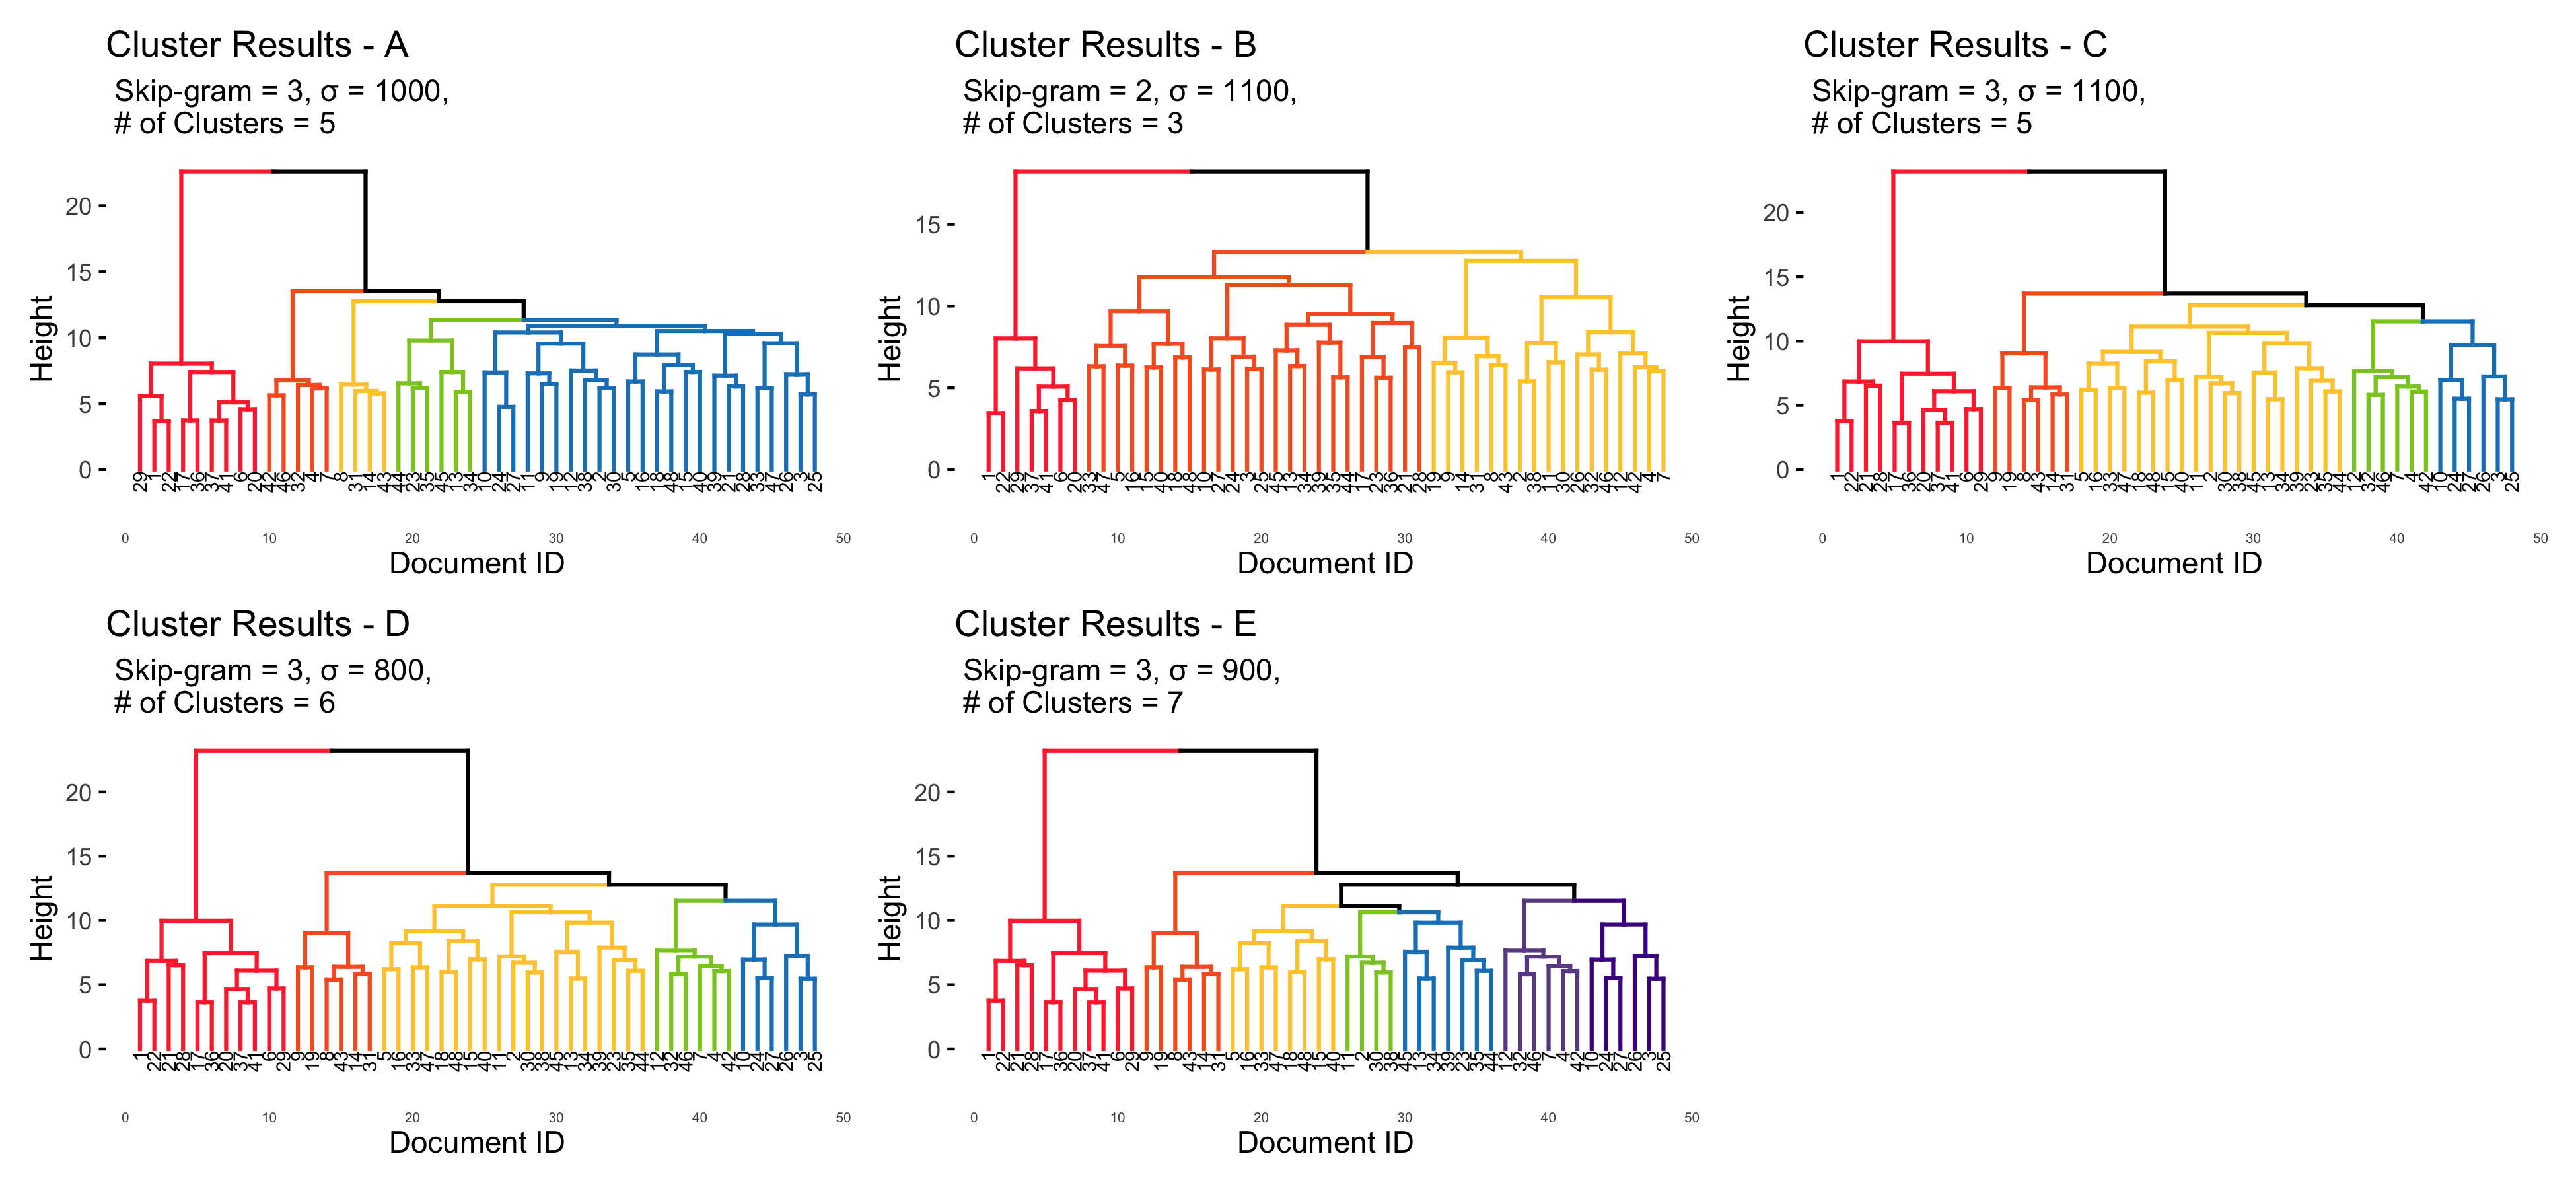
\includegraphics[width=6in]{Content/Images/5cluster.png}
\caption{Five hyper-parameter sets and their corresponding dendrograms.}
\end{figure}

To compare how often this co-membership in groups was appearing, a matrix of co-membership was created. In Figure 4.3, we see that each document has a set of other documents with which it is always clustered with, regardless of hyper-parameter configurations. These small document sets are the document sets which we can expect to have the most in common with one another.\\

\begin{figure}
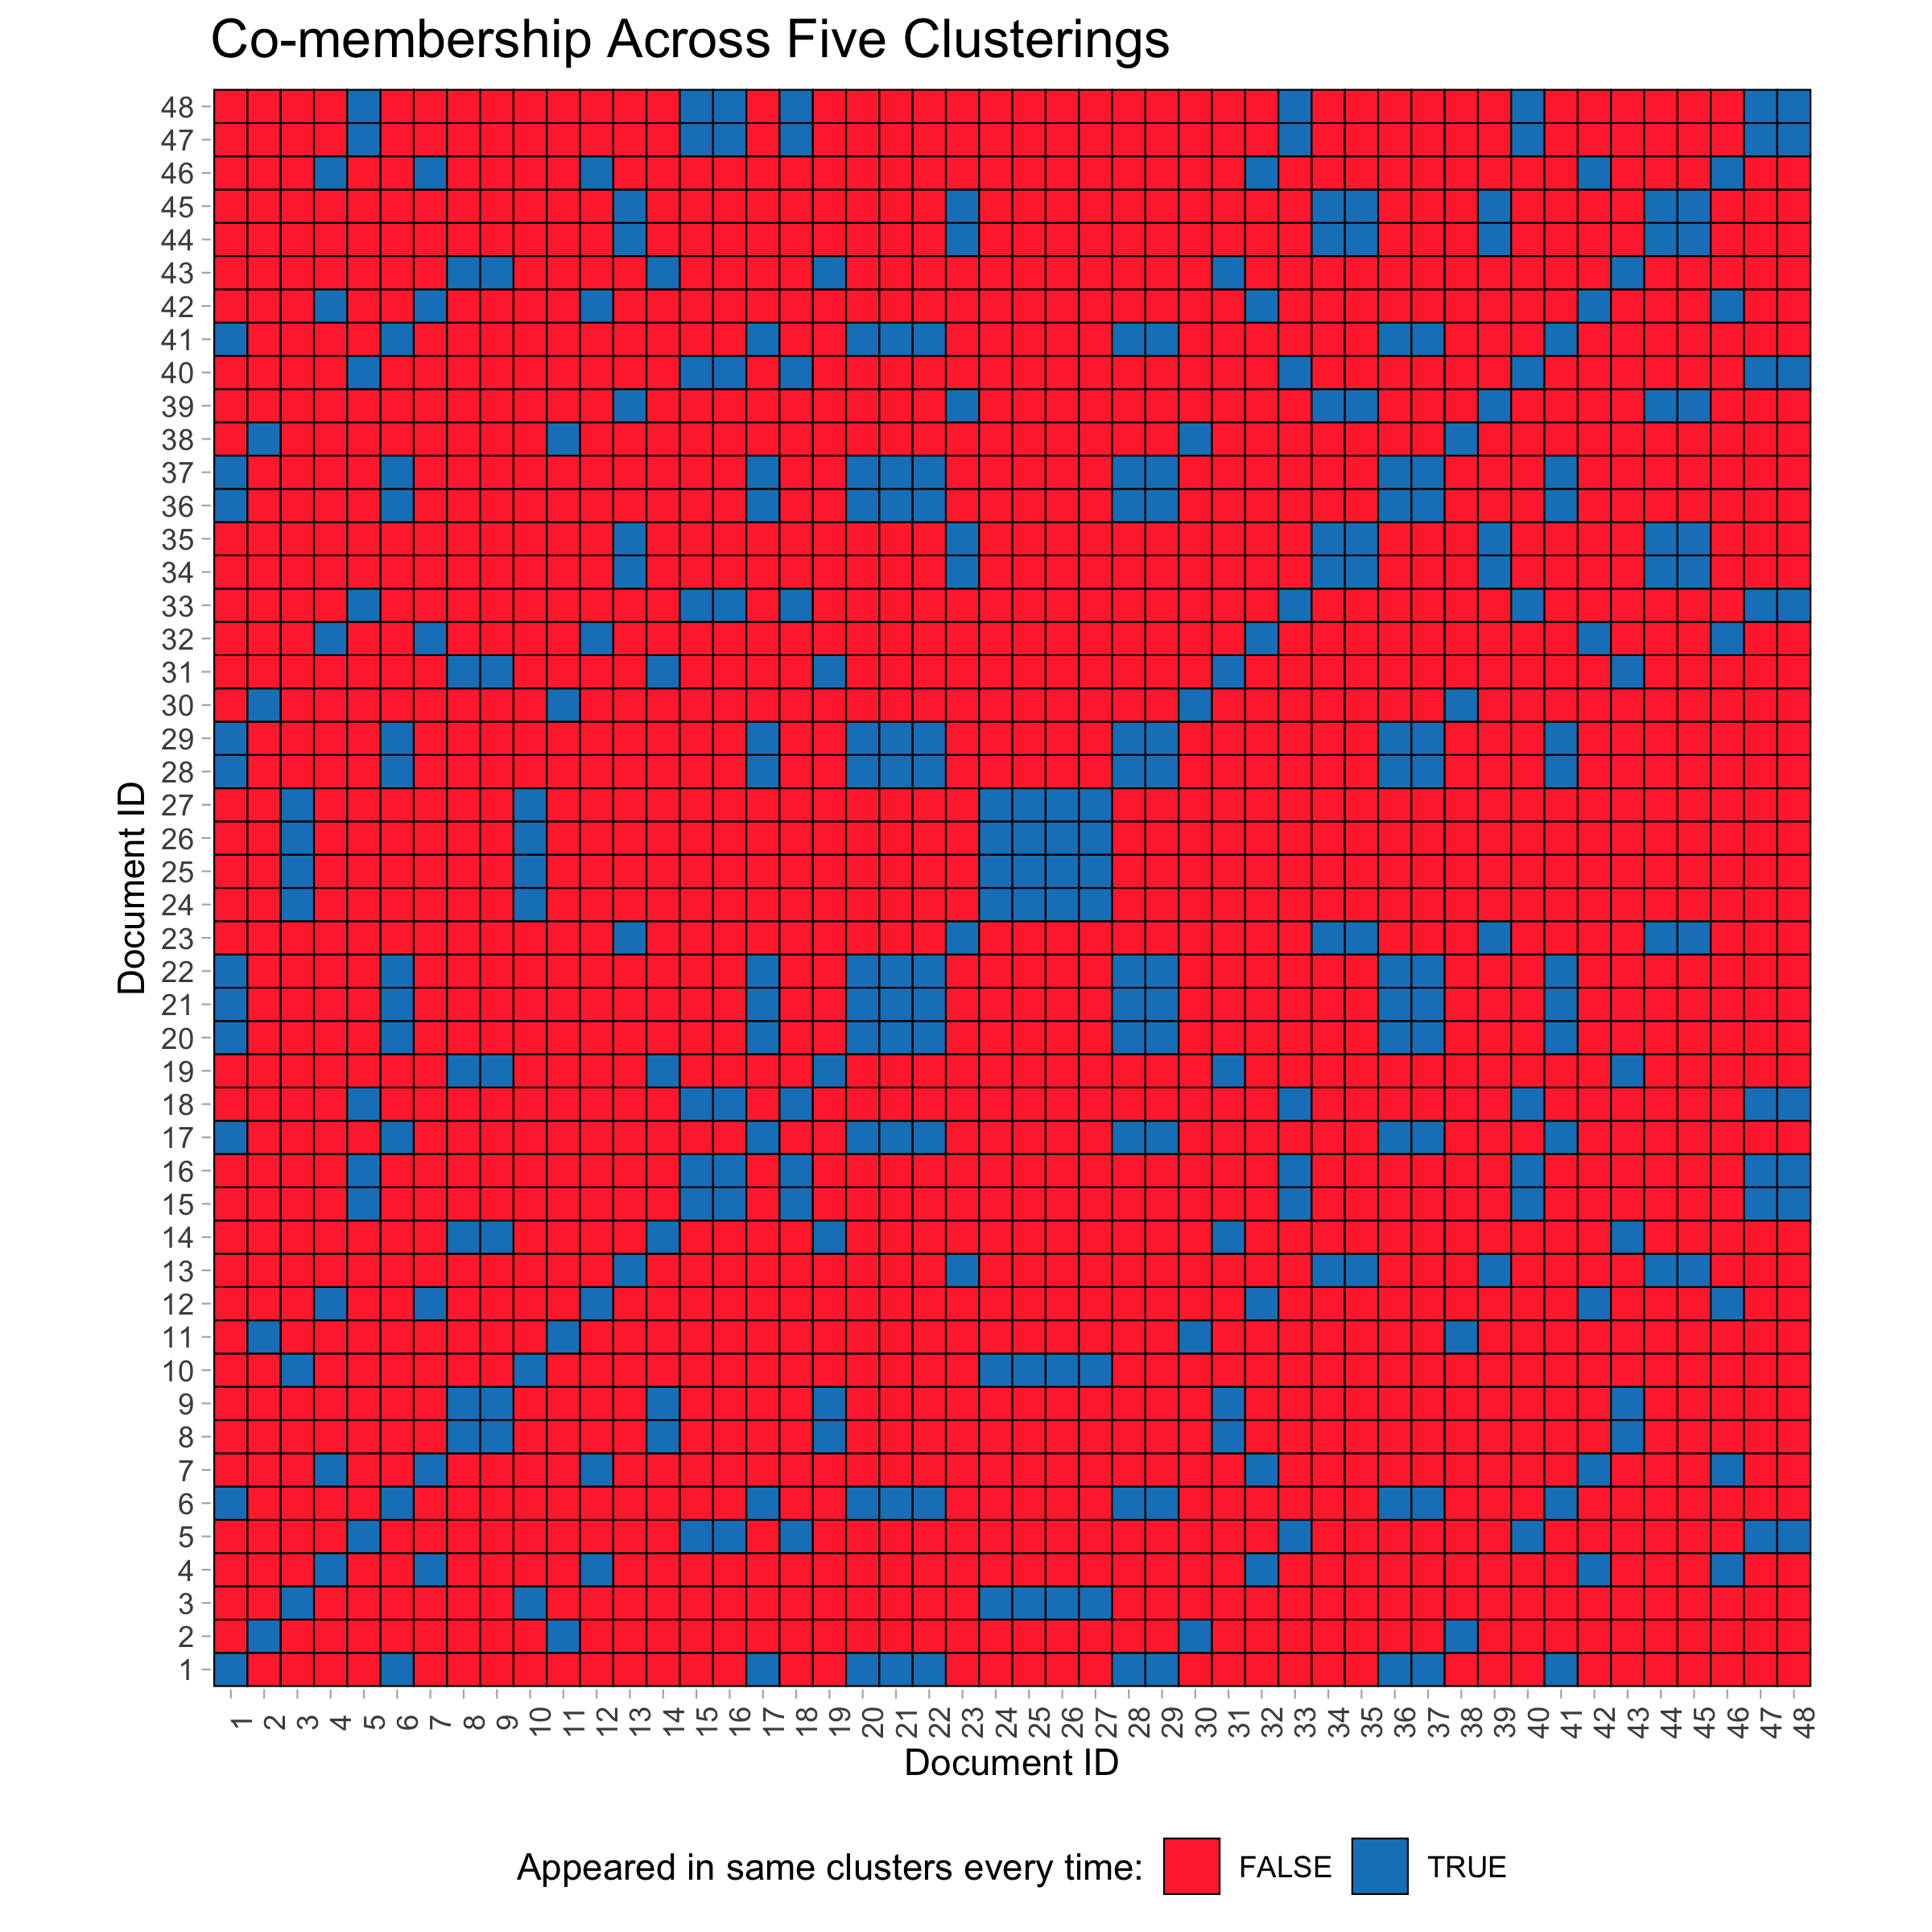
\includegraphics[width=6in]{Content/Images/comembers5.png}
\caption{Co-membership of documents across hyper-parameter sets A,B,C,D, and E.}
\end{figure}

We can inspect the results by checking some of the co-members' text. For example, document two (which was an ambulance crash in Angola, Delaware), has only 3 other co-members. Document two's co-members are: document 11, document 30, and document 38. Document 11 was an ambulance crash in Sheridan, Indiana. Document 30 was an ambulance crash in Pasadena, California. Document 38 was an ambulance crash in Ocilla, Georgia.\\
Now, we can examine some information about these four incidents that may explain their clustering. For example, all of these incidents had fatalities, three of them had roll over events, and these four were all front end collisions to the ambulance where they struck another vehicle, or object, head on. While this is just one example of the clustering methods identifying similarities in the text, we can examine similarities across the dataset through use of term-frequency/inverse document frequency.\\

\begin{equation}
\frac{tf}{idf} = \frac{\frac{\text{Term Frequency in Document}}{\text{Total Words in Document}}}{log_2(\frac{\text{Total Documents in Corpus}}{Documents with Term})}
\end{equation}

\begin{figure}
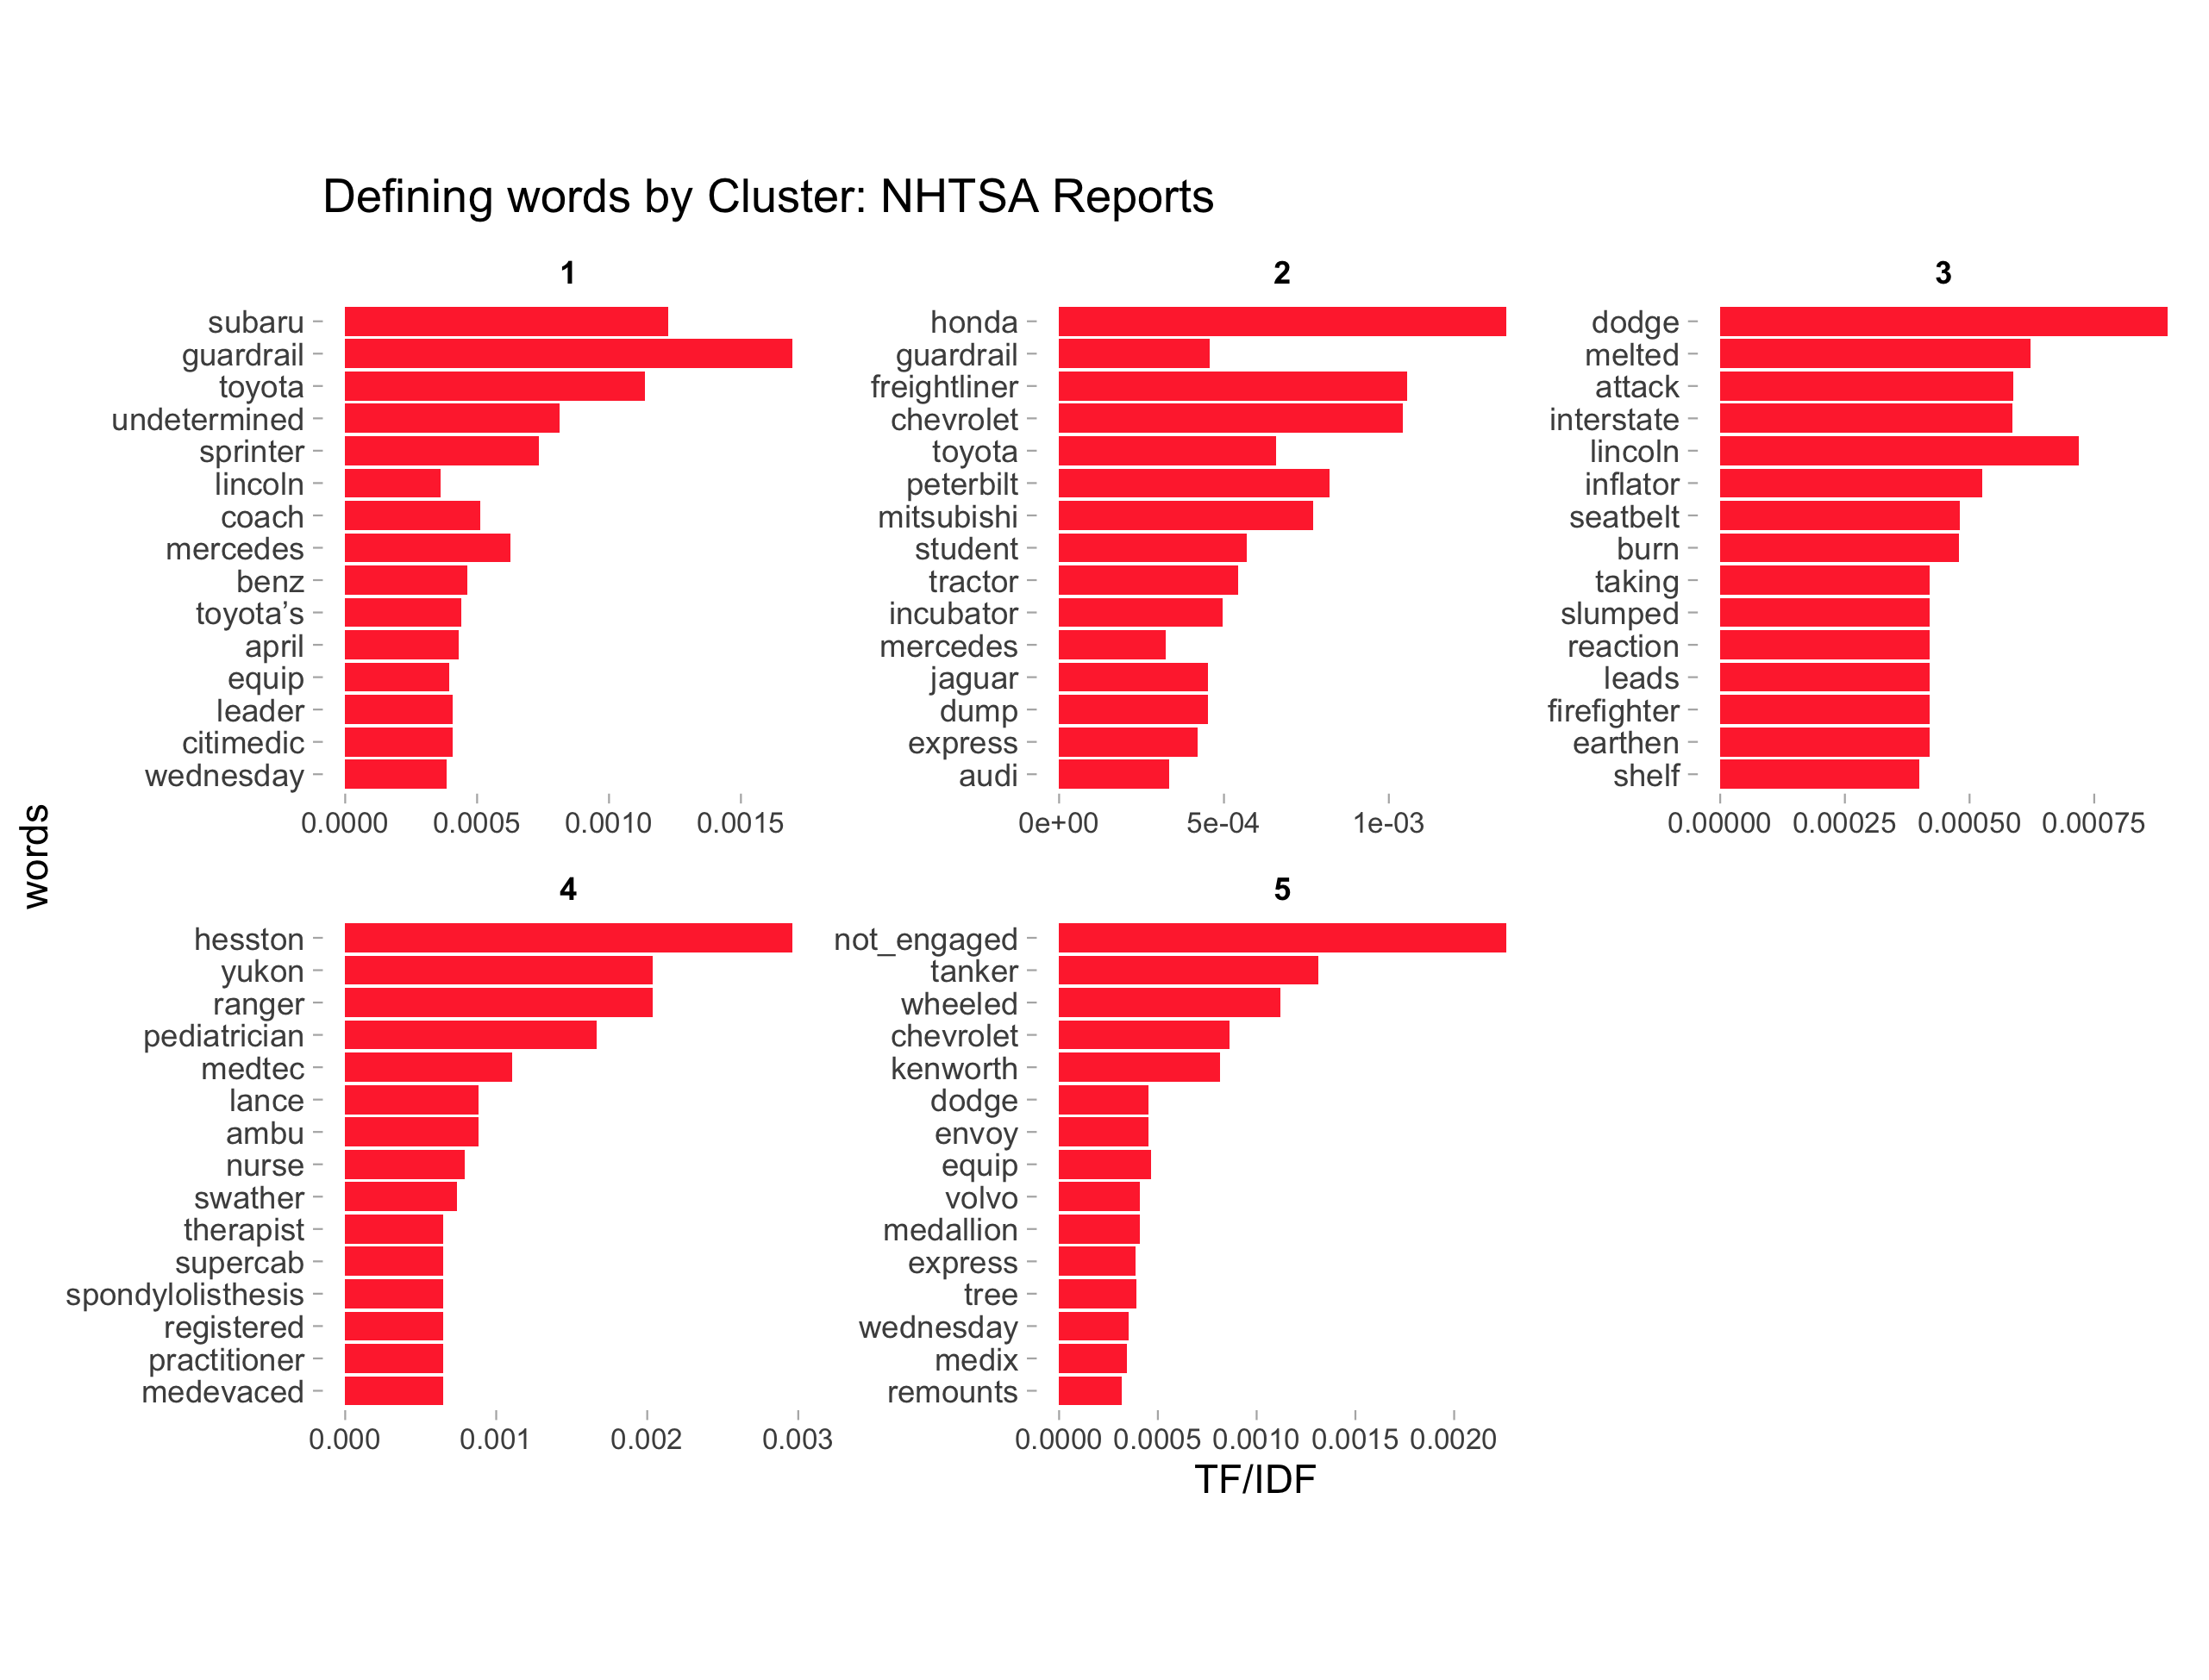
\includegraphics[width=6in]{Content/Images/nhtsa_tf_idf.png}
\caption{Term-Frequency/Inverse Document-Frequency for NHTSA reports, using hyper parameter set A.}
\end{figure}

In Figure 4.4, we see that words that appear frequently, and are unique to that cluster appear to be vehicle manufacturers, medical terms, and words that describe a crash situation (e.g. guardrail, tree, interstate). We can use these to get an idea of the crash situation. Alternatively, we can also examine portions of the skip-gram graph produced, which was used for the graph kernel calculation. \\

\begin{figure}
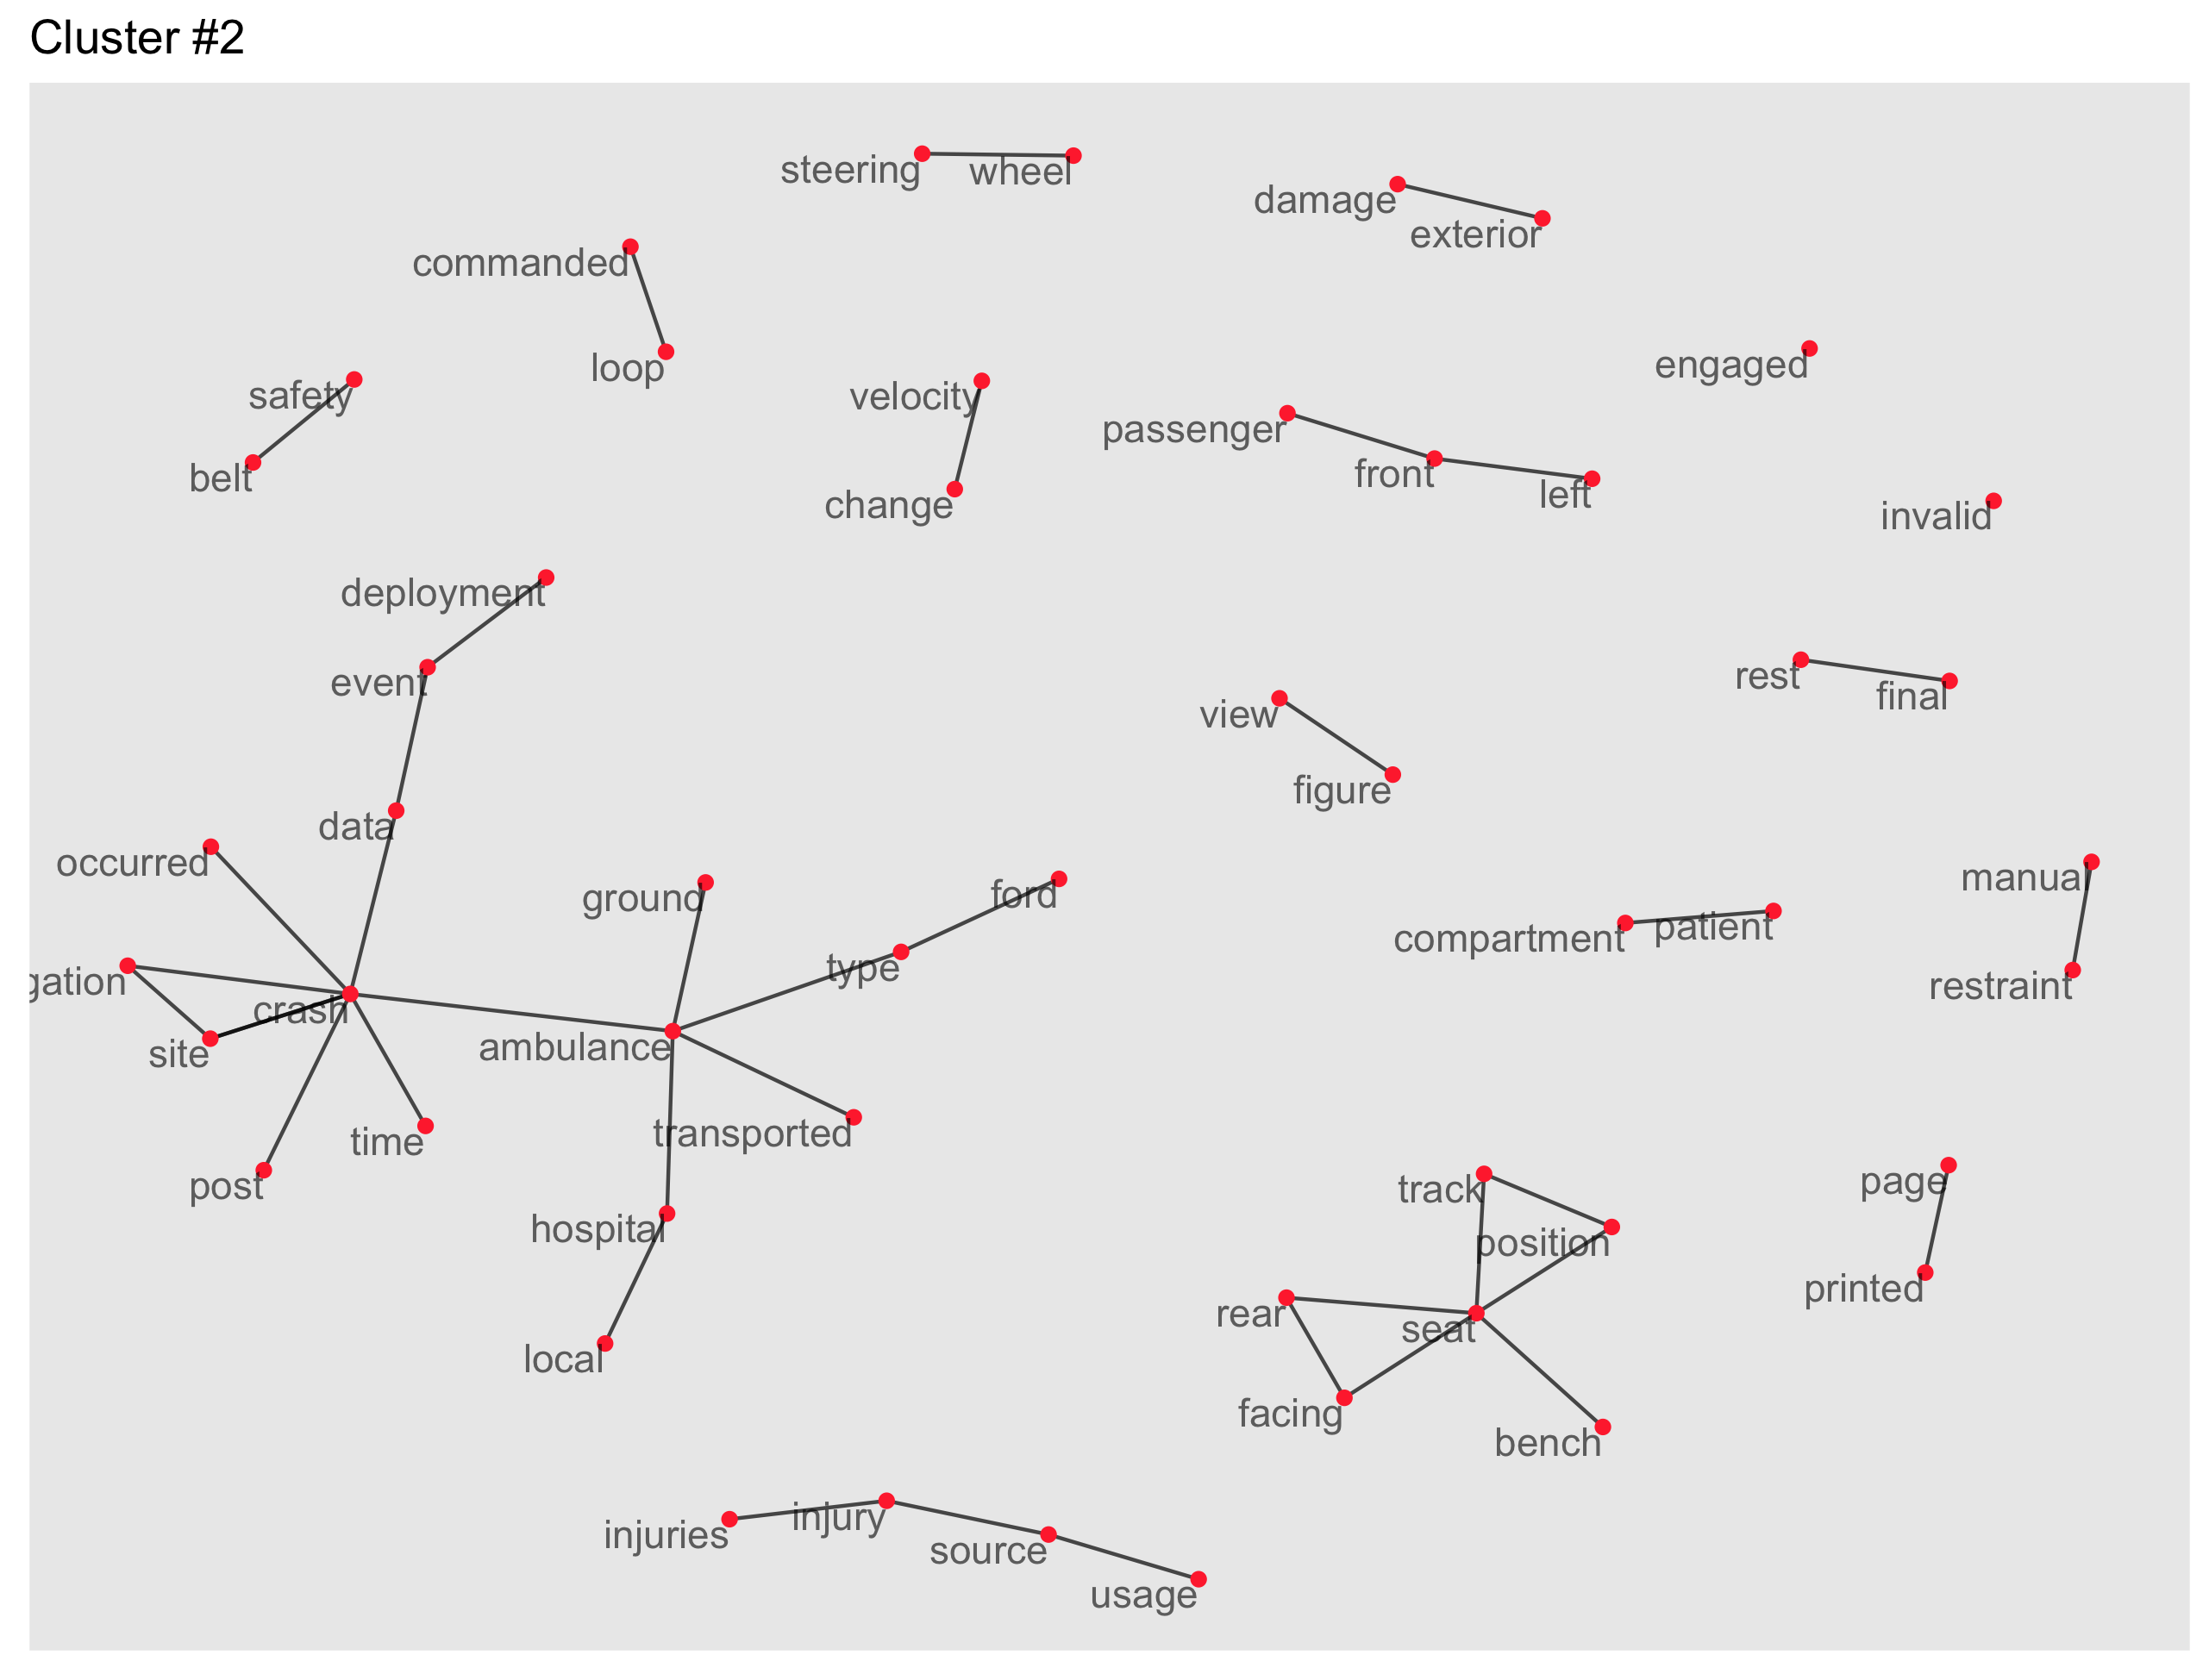
\includegraphics[width=6in]{Content/Images/graph_k5_2.png}
\caption{Skip-grams which occurred more than 50 times in hierarchical clustering with hyper-parameter set A, in cluster 3.}
\end{figure}

We can put together some of the ideas and topics discussed in the cluster. For example, in Figure 4.5 we see that ``Front Left Passenger", ``Rear Facing Seat", and ``Patient Compartment" are all skip-grams which appeared frequently in this cluster.\\


\section{reddit Threads}

For the reddit threads dataset, analysis was focused on the ability of the clusterings to organize threads based on their query words. The words used to query the \texttt{r/MentalHealth} subreddit (\texttt{https://www.reddit.com/r/mentalhealth}) all returned threads which were then clustered into new groups. Some of these clusters expressed strong preference for posts that corresponded with specific key words. \\
This data was collected with the \texttt{\{redditExtractoR\}} package \cite{rivera2015package}, and then we augmented and cleaned \texttt{\{tidytext\}} \cite{silge2016tidytext}, and other \texttt{\{tidyverse\}} tools \cite{wickham2019welcome}. These tools made it easy to extract the data from reddit, tidy the data, and perform text processing tasks such as tokenization and parsing for punctuation or numbers. Once the data was in a clean format, it followed the script map to get to a format where it could be analyzed in the same fashion as the NHTSA data was. Since this data was a large set, it utilized the scripts set up with \texttt{\{furrr\}} \cite{bengtsson2020unifying}.
To assess how many clusters to use, an ``elbow blot" was formed similar to those in Figure 4.1. For the reddit threads, the hyper parameters from the NHTSA analysis were used, and the consistently lowest metric parameter set was chosen; skip-grams of $k=3$ and kernel parameter $\sigma = 1200$ were used in the reddit clustering analysis. In Figure 4.6, we see that 4 clusters is the optimal value, where additional clusters provides diminishing results. \\

\begin{figure}
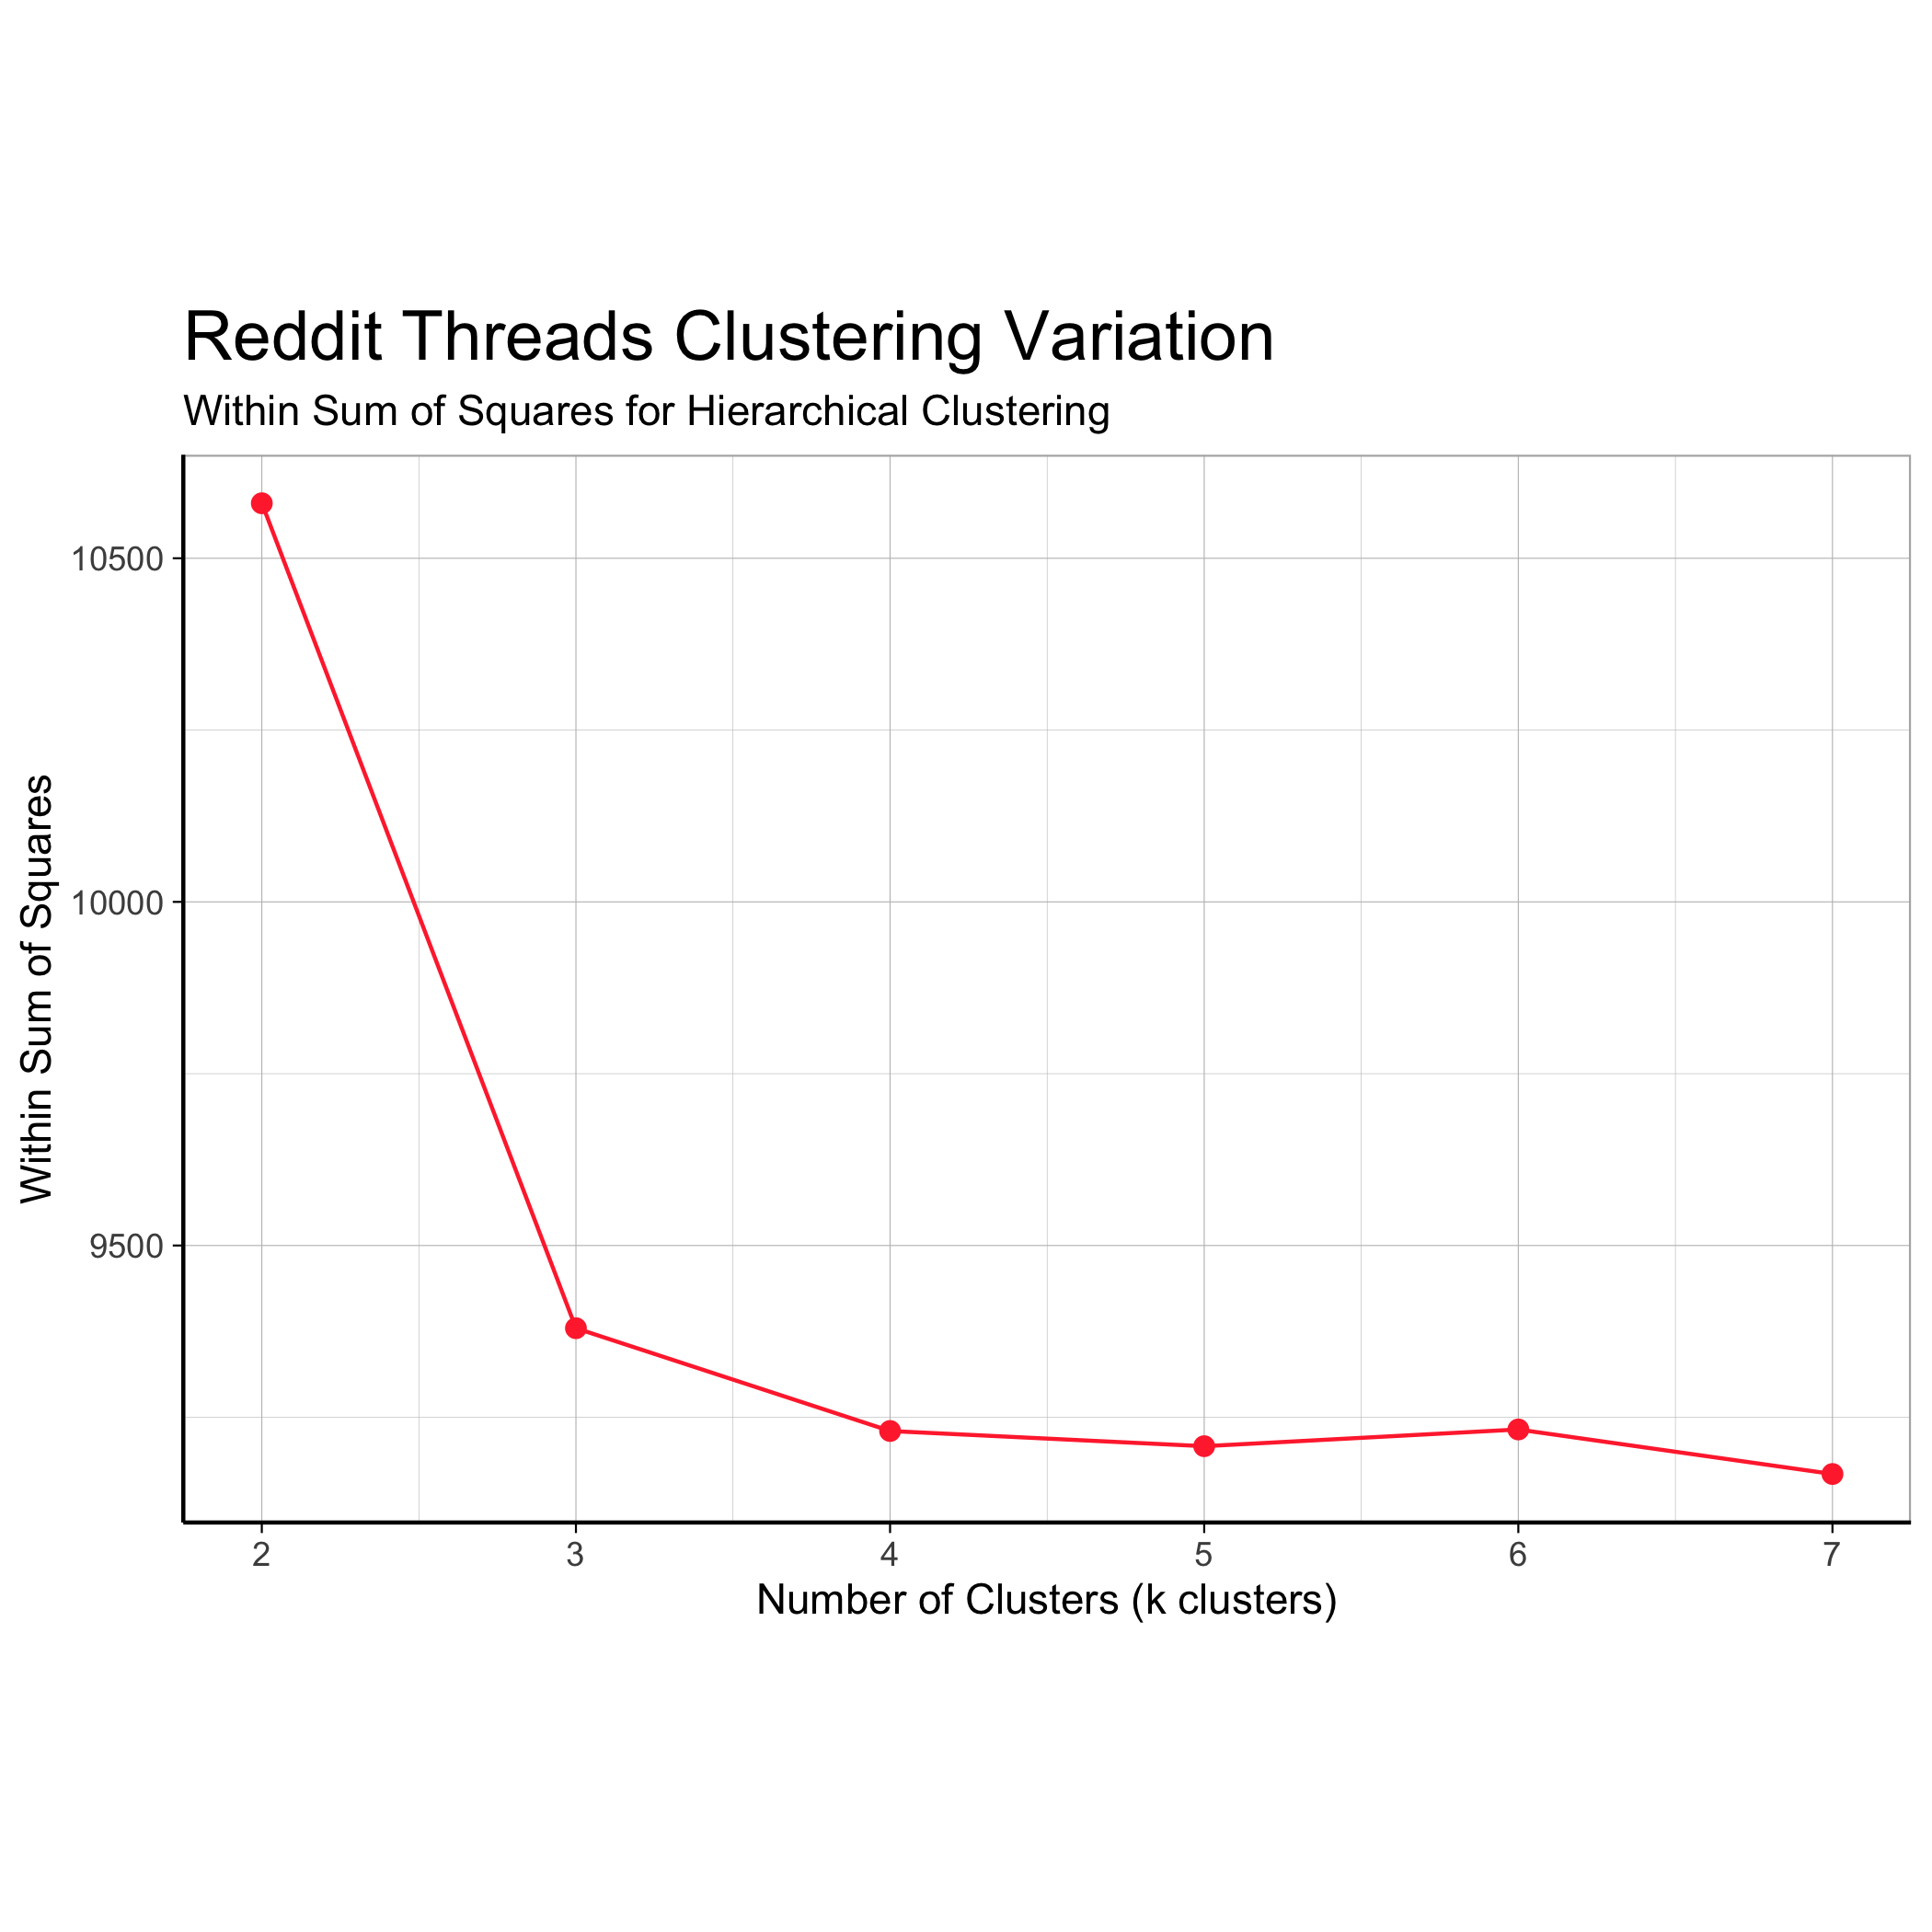
\includegraphics[width=6in]{Content/Images/reddit_wss.png}
\caption{Within sum of squares as a function of number of clusters}
\end{figure}

After computing the kernel and using these parameters, four cluster are produced. Examining the dendrogram, in Figure 4.7, we see that we have 2 very distinct groups, which then break into two smaller groups. These groups are very clear and provide confidence in the clustering results. Along side the dendrogram, there is a heat map of what proportion of documents (or threads) in the cluster came from a query word. In Figure 4.7, we see that clusters 3 and 4 collected posts from the "angry" query word. Additionally cluster 1 displays a 
strong amount of its posts coming from the "sad" query word. \\

\begin{figure}
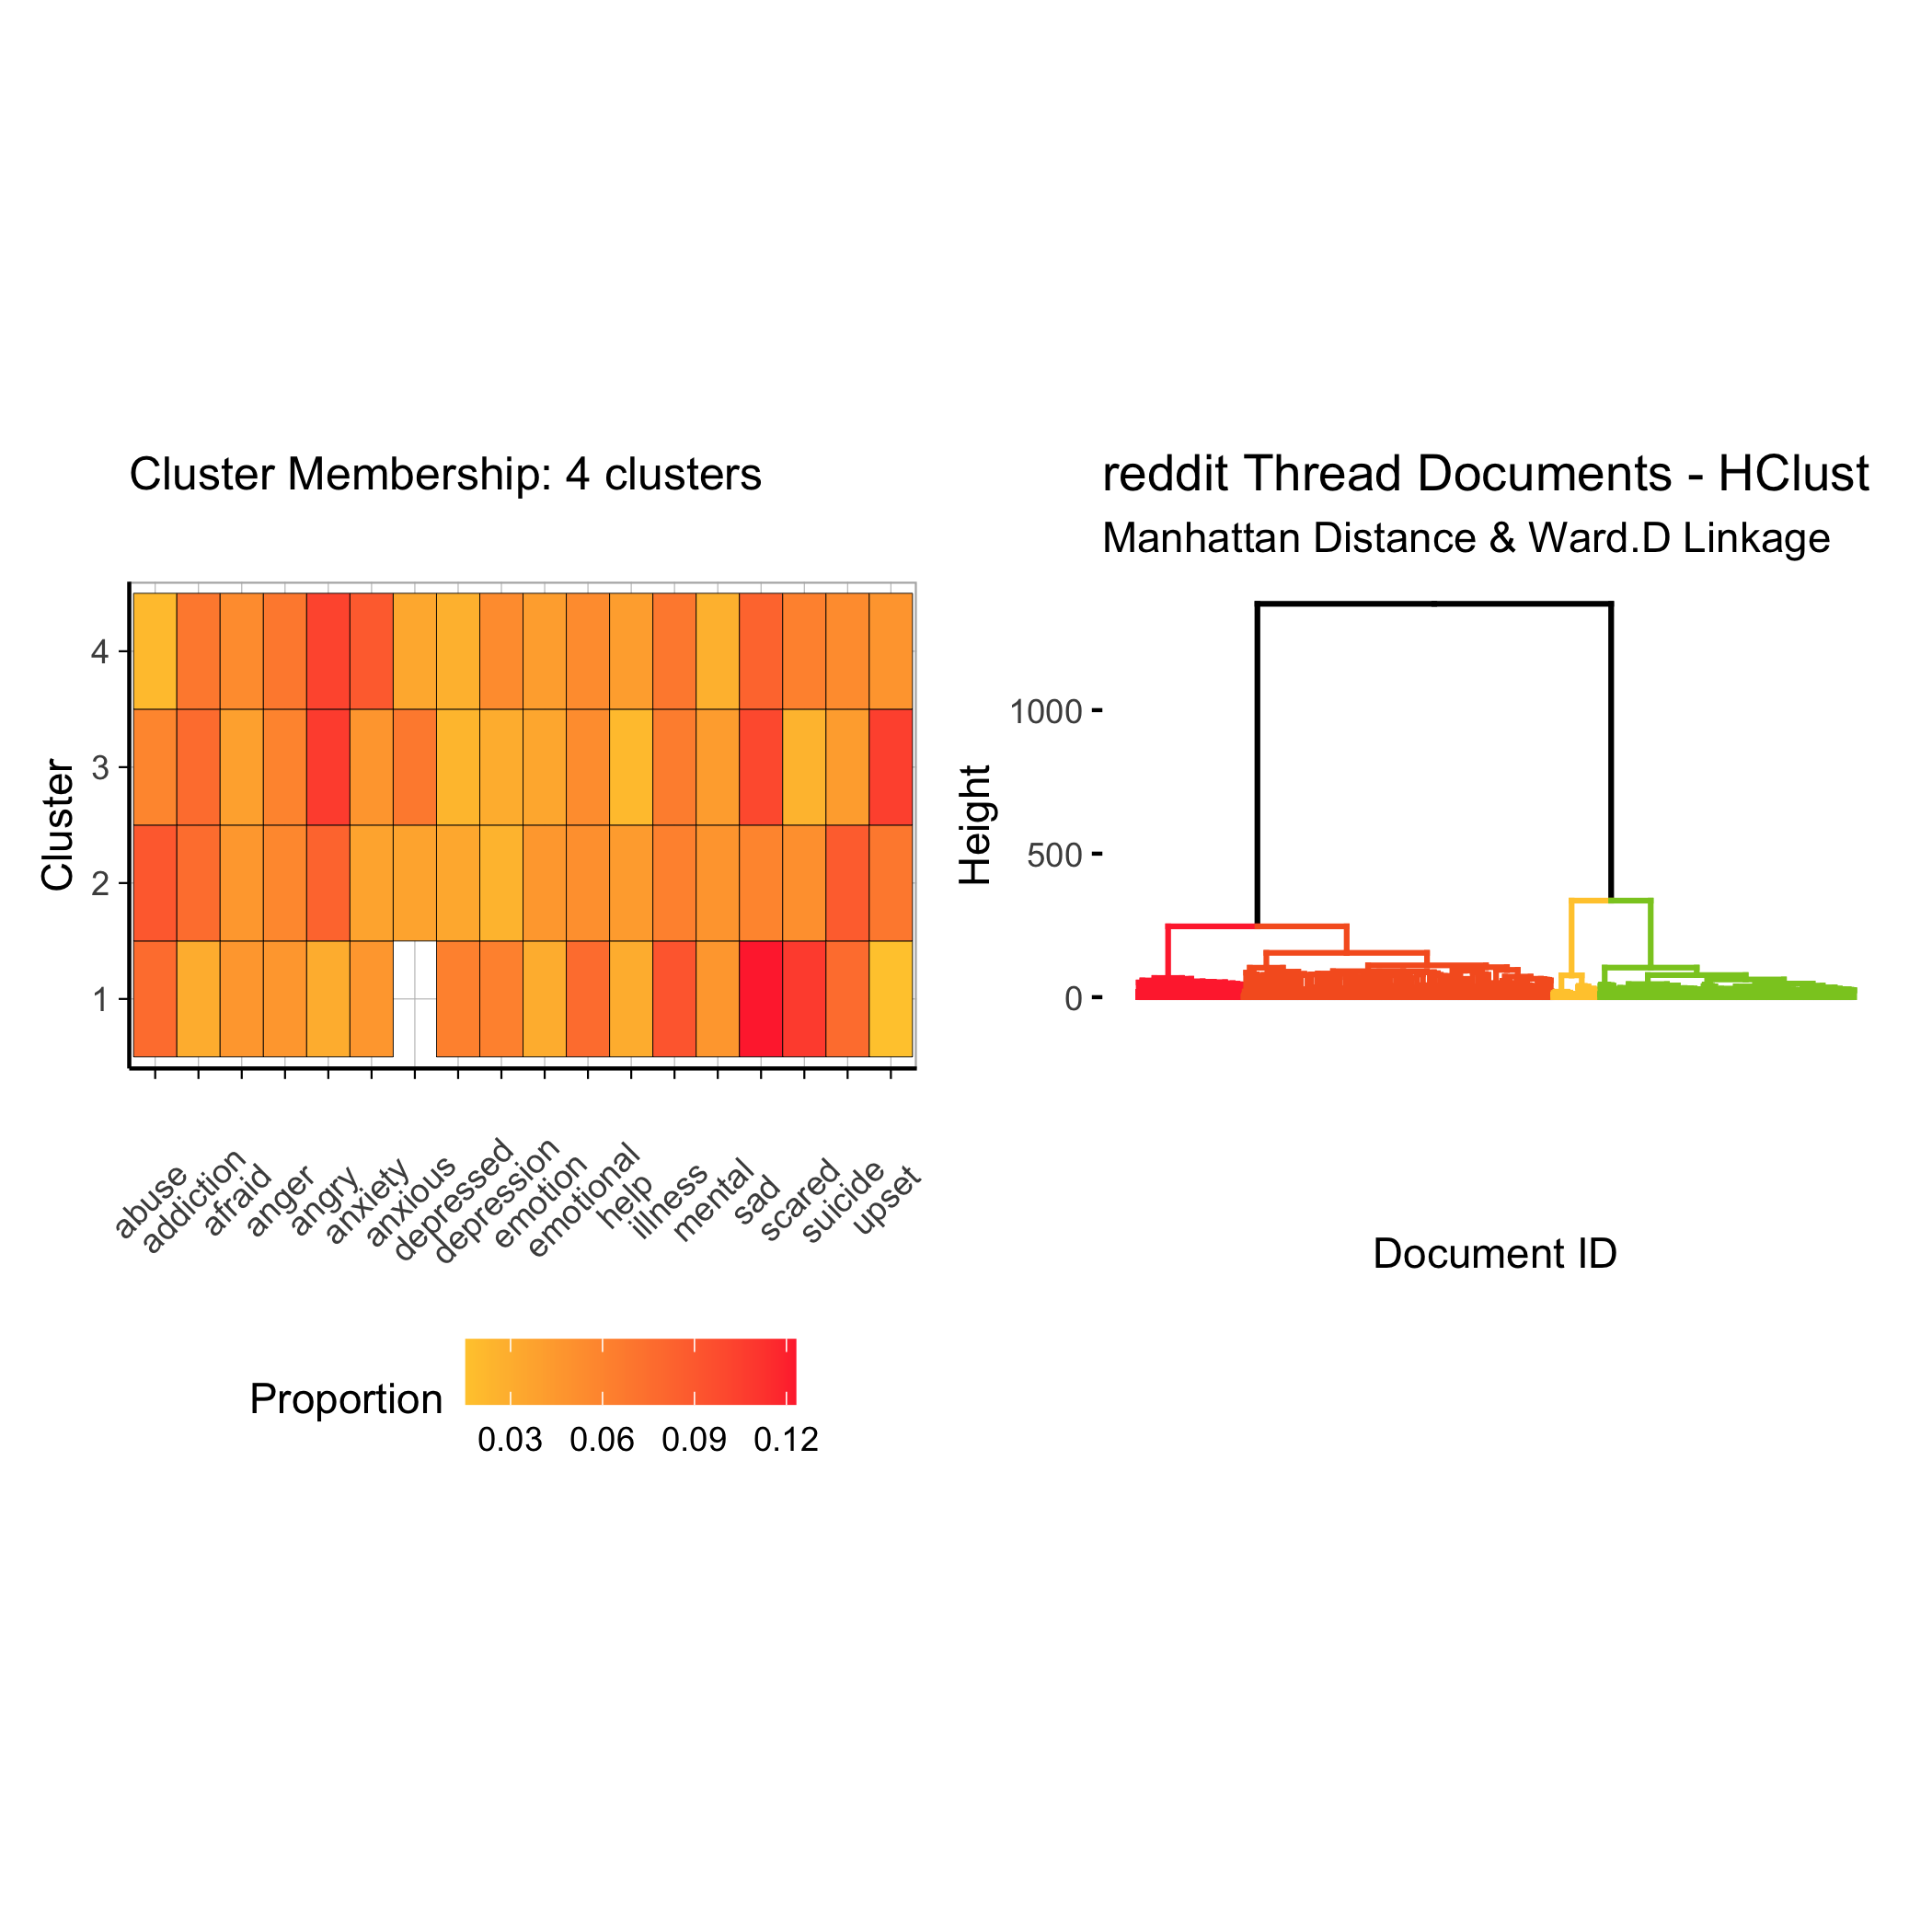
\includegraphics[width=6in]{Content/Images/k4_reddit_clusters.png}
\caption{Left - Proportion of cluster's threads coming from each query word. Right - Dendrogram for reddit thread analysis, with 4 clusters.}
\end{figure}

The prominence of some of these query words in the clusters indicates that the tone or language used by the thread authors was picked out by the clustering methods. This is of particular interest, as the goal of these methods was to perform unsupervised text clustering which utilized more of the rich intricacies of language.\\

\section{Comparative Analysis}

Looking at the results from both hierarchical clusterings on the graph kernels it is apparent that these methods work much better on larger documents. The performance of the graph kernels being applied to the skip-gram graph and then clustering was much better in the NHTSA dataset than the reddit threads dataset. By measuring within sum of squares, the NHTSA data set performed much better, and the computation time was much smaller despite the documents being substantially longer than the reddit comments. However, the reddit dataset displayed more prominent clusters, which was also indicative of success.\\
Comparing the elbow plots for both the NHTSA and the reddit threads datasets, it is clear that the optimal number of clusters for these methods will be dependent upon the dataset being analyzed. The results from the NHTSA study that indicated that skip-grams with $k=3$ did seem to apply to the reddit dataset as well. These hyper parameters will need tuning for any new application.\\
Overall, the largest difference between the two analyses was that although the reddit threads displayed strong, prominent clusters, the NHTSA dataset was being computed in reasonable amount of time. Since the application of these methods are scaling better for increasing document size instead of increasing document lists, there is a case to be made that aggregating reddit threads into larger documents may be more effective, but to keep the observational unit tied to a reddit thread, this was not completed.\\ 
These methods could be applied in any smaller text mining application. Since the methods were able to be parallelized during their most computationally expensive portions of code, the methods could scale with sufficient hardware. In a high performance computing environment, with a much larger dataset, it may become clear that these methods are either more effective or less effective than they were found to be here.


 

 


